\documentclass[UTF8]{ctexart}
\usepackage[a4paper,left=3cm,right=3cm,top=2cm]{geometry}
\usepackage{amsmath}
\usepackage{enumitem}
\usepackage{float}
\usepackage{threeparttable}
\usepackage{caption}
\usepackage{multirow}
\usepackage{graphicx}
\usepackage{listings}
\usepackage{color}
\definecolor{dkgreen}{rgb}{0,0.6,0}
\definecolor{gray}{rgb}{0.5,0.5,0.5}
\definecolor{mauve}{rgb}{0.58,0,0.82}
\lstset{frame=tb,
  language=Python,
  aboveskip=3mm,
  belowskip=3mm,
  showstringspaces=false,
  columns=flexible,
  basicstyle={\small\ttfamily},
  numbers=left,%设置行号位置none不显示行号
  %numberstyle=\tiny\courier, %设置行号大小
  numberstyle=\tiny\color{gray},
  keywordstyle=\color{blue},
  commentstyle=\color{dkgreen},
  stringstyle=\color{mauve},
  breaklines=true,
  breakatwhitespace=true,
  escapeinside=`,%逃逸字符(1左面的键),用于显示中文例如在代码中`中文...`
  tabsize=4,
  extendedchars=false %解决代码跨页时,章节标题,页眉等汉字不显示的问题
}

\setlength\lineskiplimit{5.25bp}
\setlength\lineskip{5.25bp}

\title{霍尔效应实验报告}
\author{崔士强 PB22151743}
\date{\today}

\bibliographystyle{plain}

\begin{document}

\maketitle
\section{实验目的}
本实验的目的是通过用霍尔元件测量磁场,判断霍尔元件载流子类型,计算载流子的浓度和迁移速度,以及了解霍尔效应测试中的各种副效应及消除方法.
\section{实验原理}
\subsection{霍尔系数的测量}
\begin{figure}[h]
  \centering
  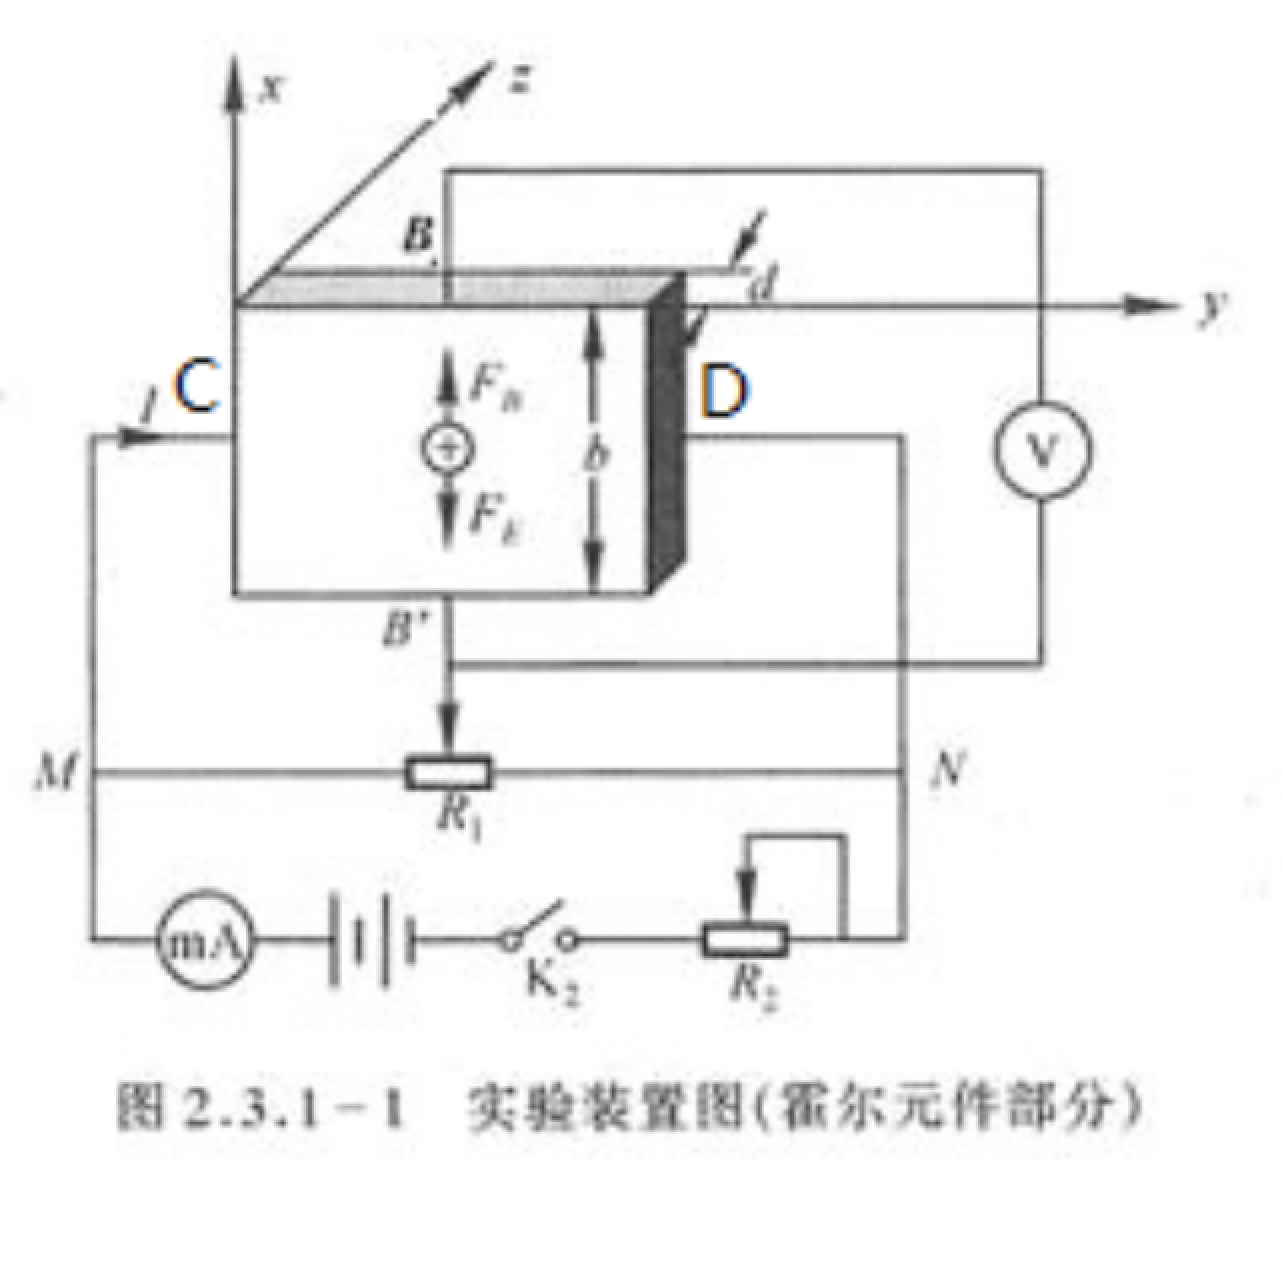
\includegraphics[scale=0.3]{p1.png}
  \caption{实验原理}
\end{figure}
如图所示,半导体片与电路连接,当$y$方向有电流$I_S$时,半导体片中的载流子受洛伦兹力$F_B$作用,向$x$方向偏移. 设载流子运动速度为$u$,
则有:
\[F_B = quB\]

随着电荷累积,薄片$B$, $B'$两侧产生电场$E$,设电场力为$F_E$,则有:
\[F_E = \frac{qV_{BB'}}{b}\]

平衡时有$F_E = F_B$,即:
\[quB = \frac{qV_{BB'}}{b}\]

设载流子浓度为$n$,有:
\[I_S = bdnqu\]

从而得到
\[V_{BB'} = \frac{1}{nq}\frac{I_SB}{d}\]

令霍尔系数$R_H = \frac{1}{nq}$, 则:
\[V_{BB'} = R_H\frac{I_SB}{d}\]

已知磁铁线圈参数为:$ \frac{B}{I_M} = 3600\mathrm{Gs/A} = 0.36\mathrm{T/A}$,则可以通过$I_S$或$I_M$
与$V_{BB'}$的关系来测量$R_H$. 在本实验中,为了减少副效应,采取对称测量法,即对于每一组$I_S$和$I_M$的值,分别换向从而测得四组电压值,取其平均值.
\subsection{电导率的测量}
沿电流方向测量一段距离$L$两端的电压,则有:
\[\frac{V}{I_S} = \rho \frac{L}{bd}\]

即可计算出电导率. 已知电导率与载流子浓度$n$,迁移率$\mu$ 之间的关系:
\[\sigma = ne\mu\]

则可以计算出载流子浓度$n$以及迁移率$\mu$.
\subsection{载流子类型的确定}
无论是正电荷还是负电荷,其偏转方向是一致的,因此测量半导体$x$方向两端电压即可得知载流子类型.         
\section{实验仪器}
恒流源,电磁铁,霍尔样品和样品架,锑化铟片,换向开关和接线柱,数字万用表,小磁针.
\section{测量记录}
\subsection{测量六角霍尔片的霍尔系数}
\begin{minipage}[c]{0.5\textwidth}
  \centering
  \begin{tabular}{ccc}
    \hline\hline
    \multirow{2}*{$I_S(\mathrm{mA})$} & \multicolumn{2}{c}{$I_M(\mathrm{A})$} \\
    \cline{2-3}
    ~ & $+0.45$ & $-0.45$ \\
    \hline
    $+1.00$ & 2.100 & 1.984 \\
    $-1.00$ & 2.096 & 1.983 \\
    $+1.50$ & 3.146 & 2.957 \\
    $-1.50$ & 3.143 & 2.958 \\
    $+2.00$ & 4.178 & 3.929 \\
    $-2.00$ & 4.177 & 3.930 \\
    $+2.50$ & 5.170 & 4.864 \\
    $-2.50$ & 5.165 & 4.865 \\
    $+3.00$ & 6.207 & 5.839 \\
    $-3.00$ & 6.202 & 5.840 \\
    $+3.50$ & 7.241 & 6.814 \\
    $-3.50$ & 7.225 & 6.816 \\
    $+4.00$ & 8.278 & 7.791 \\
    $-4.00$ & 8.271 & 7.792 \\
    $+4.50$ & 9.316 & 8.764 \\
    $-4.50$ & 9.314 & 8.766 \\
    \hline\hline
  \end{tabular}
  \captionof{table}{固定$I_M$所得电压$V_{BB'}$}
\end{minipage}
\begin{minipage}[c]{0.5\textwidth}
  \centering
  \begin{tabular}{ccc}
    \hline\hline
    \multirow{2}*{$I_M(\mathrm{A})$} & \multicolumn{2}{c}{$I_S(\mathrm{mA})$} \\
    \cline{2-3}
    ~ & $+4.5$ & $-4.5$ \\
    \hline
    $+0.100$ & 2.141 & 2.151 \\
    $-0.100$ & 1.606 & 1.605 \\
    $+0.150$ & 3.060 & 3.097 \\
    $-0.150$ & 2.548 & 2.546 \\
    $+0.200$ & 4.020 & 4.070 \\
    $-0.200$ & 3.519 & 3.520 \\
    $+0.250$ & 5.007 & 5.076 \\
    $-0.250$ & 4.531 & 4.529 \\
    $+0.300$ & 6.018 & 6.130 \\
    $-0.300$ & 5.582 & 5.581 \\
    $+0.350$ & 7.095 & 7.172 \\
    $-0.350$ & 6.620 & 6.617 \\
    $+0.400$ & 8.142 & 8.224 \\
    $-0.400$ & 7.672 & 7.667 \\
    $+0.450$ & 9.209 & 9.307 \\
    $-0.450$ & 8.756 & 8.755 \\
    \hline\hline
  \end{tabular}
  \captionof{table}{固定$I_S$所得电压$V_{BB'}$}
\end{minipage}
\subsection{测量六角霍尔片的电导率}
在零磁场下,取$I_S = 1.00\mathrm{mA}$,测得$V_{B'A'} = -60\mathrm{mV}$.
\subsection{确定导电类型}
\begin{figure}[h]
  \centering
  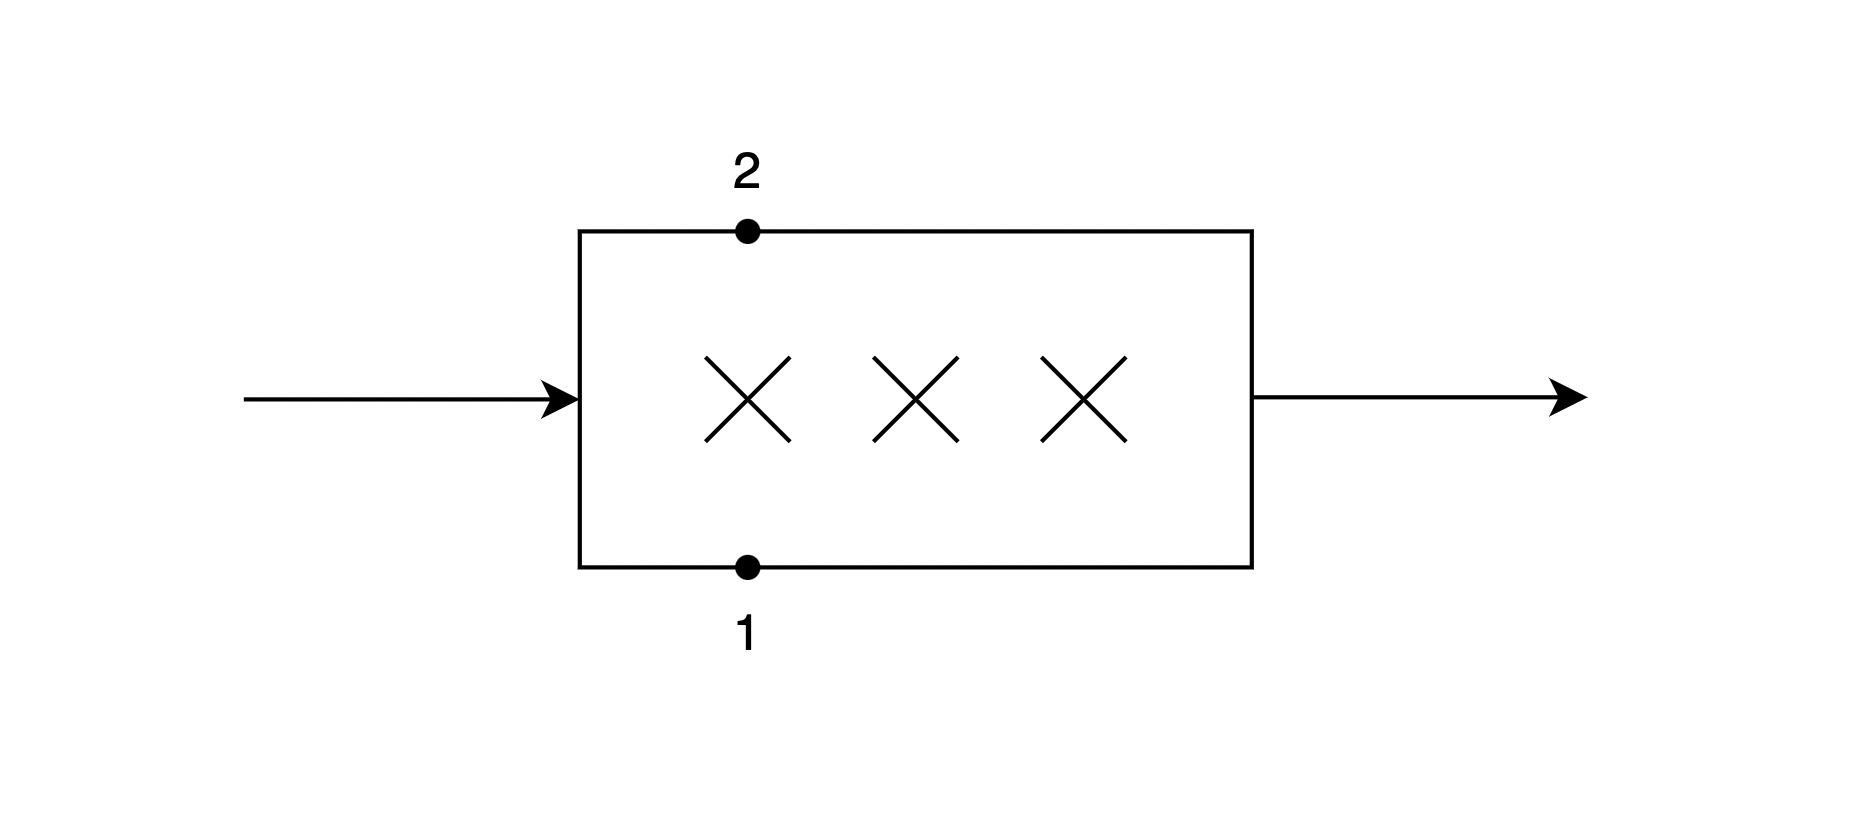
\includegraphics[scale=0.3]{p4.png}
  \caption{示意图}
\end{figure}
测得$V_{12} > 0 $

\subsection{测量锑化铟片的霍尔系数}
固定$I_S = 1\mathrm{mA}$,改变$I_M$,测得$V_{H}$如下:

\begin{table}[h]
  \centering
  \begin{tabular}{cc}
    \hline\hline
    $I_M(\mathrm{A})$ & $V_{H}(\mathrm{mV})$ \\
    \hline
    0.00 & $-60.0$ \\
    0.05 & $-20.2$ \\
    0.10 & 15.3 \\
    0.15 & 46.9 \\
    0.20 & 73.7 \\
    0.22 & 84.8 \\
    0.25 & 92.3 \\
    0.27 & 98.5 \\
    0.30 & 104.0 \\
    0.35 & 115.5 \\
    0.40 & 124.4 \\
    0.45 & 132.3 \\
    0.50 & 141.3 \\
    0.55 & 150.2 \\
    0.60 & 159.4 \\
    0.65 & 167.9 \\
    0.70 & 177.0 \\
    0.75 & 185.4 \\
    0.80 & 194.3 \\
    \hline\hline
  \end{tabular}
  \caption{固定$I_S = 1\mathrm{mA}$所得电压$V_H$}
\end{table}
\section{分析与讨论}
\subsection{数据处理}
对于4.1中的数据,求两次换向所得四个值的平均值,并作线性拟合,结果如下:

\begin{minipage}{0.5\textwidth}
  \centering
  \begin{tabular}{cc}
    \hline\hline
    $I_S(\mathrm{mA})$ & $V_{BB'}(\mathrm{mV})$ \\
    \hline
    1.00 & 2.041 \\
    1.50 & 3.051 \\
    2.00 & 4.054 \\
    2.50 & 5.016 \\
    3.00 & 6.022 \\
    3.50 & 7.024 \\
    4.00 & 8.033 \\
    4.50 & 9.040 \\
    \hline\hline
  \end{tabular}
  \captionof{table}{固定$I_M=0.45\mathrm{A}$所得电压$V_{BB'}$}
\end{minipage}
\begin{minipage}{0.5\textwidth}
  \centering
  \begin{tabular}{cc}
    \hline\hline
    $I_M(\mathrm{A})$ & $V_{BB'}(\mathrm{mV})$ \\
    \hline
    0.100 & 1.876 \\
    0.150 & 2.813 \\
    0.200 & 3.782 \\
    0.250 & 4.786 \\
    0.300 & 5.828 \\
    0.350 & 6.876 \\
    0.400 & 7.926 \\
    0.450 & 9.007 \\
    \hline\hline
  \end{tabular}
  \captionof{table}{固定$I_S=4.5\mathrm{mA}$所得电压$V_{BB'}$}
\end{minipage}

\begin{figure}[h]
  \centering
  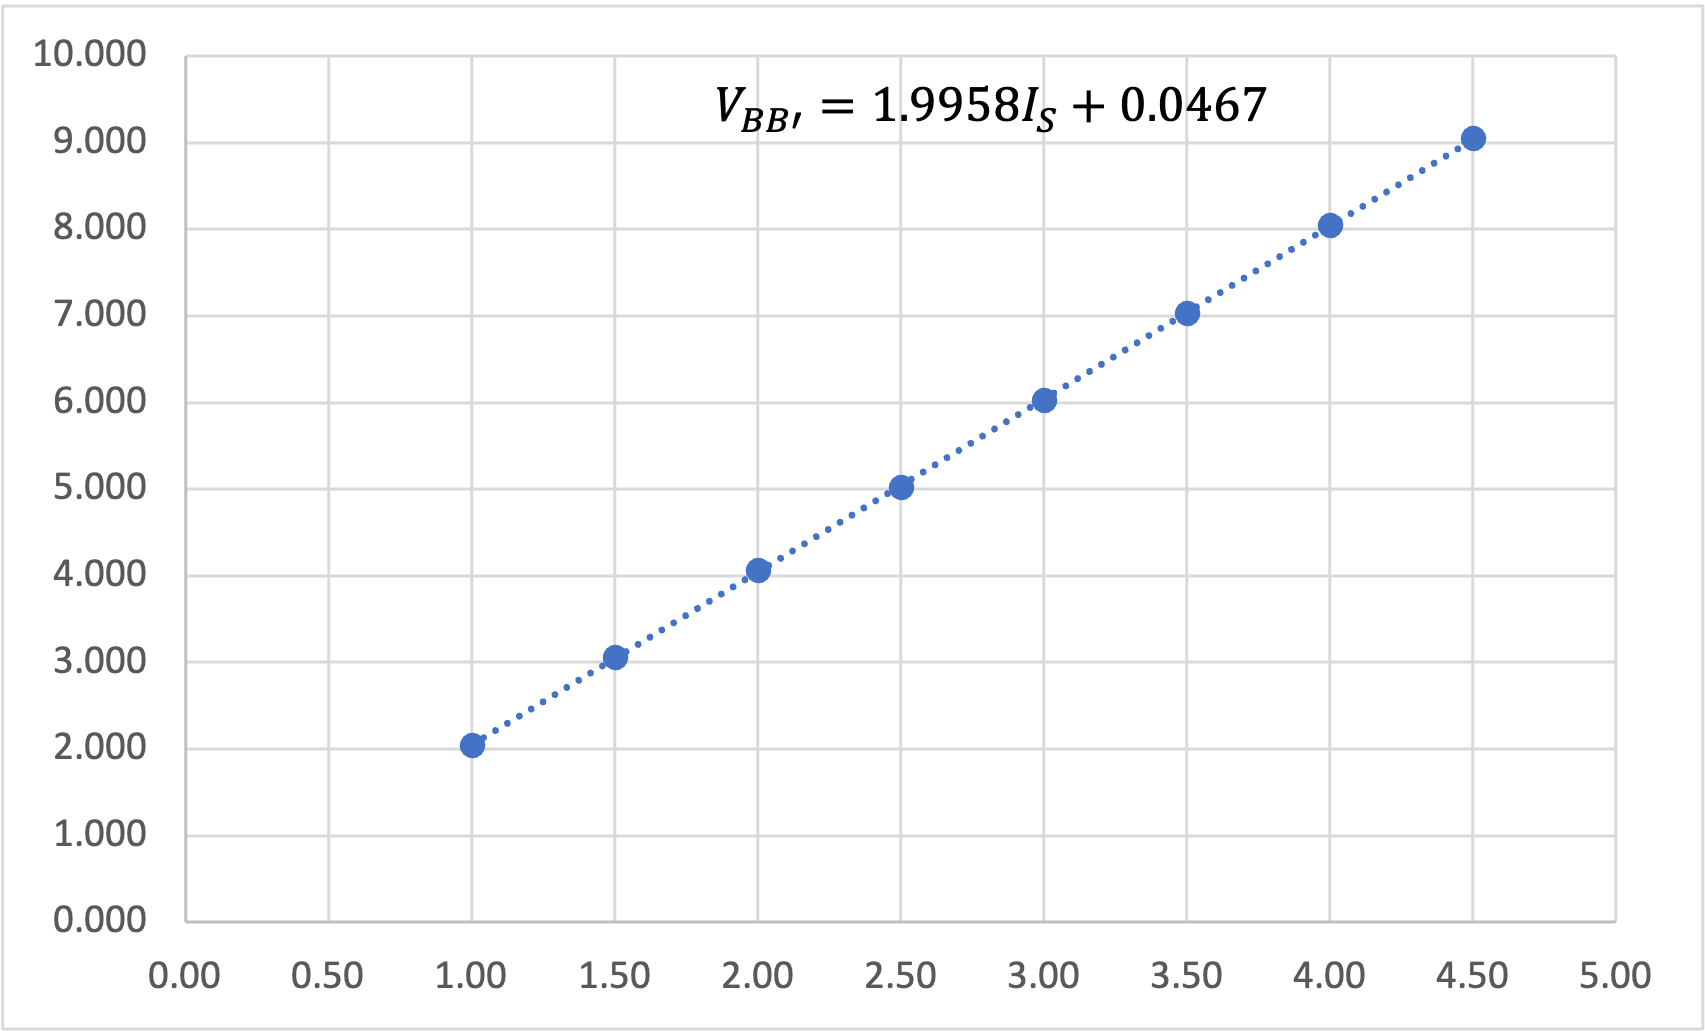
\includegraphics[scale=0.7]{p2.png}
  \caption{$V_{BB'}$与$I_S$的关系}
\end{figure}
\begin{figure}[h]
  \centering
  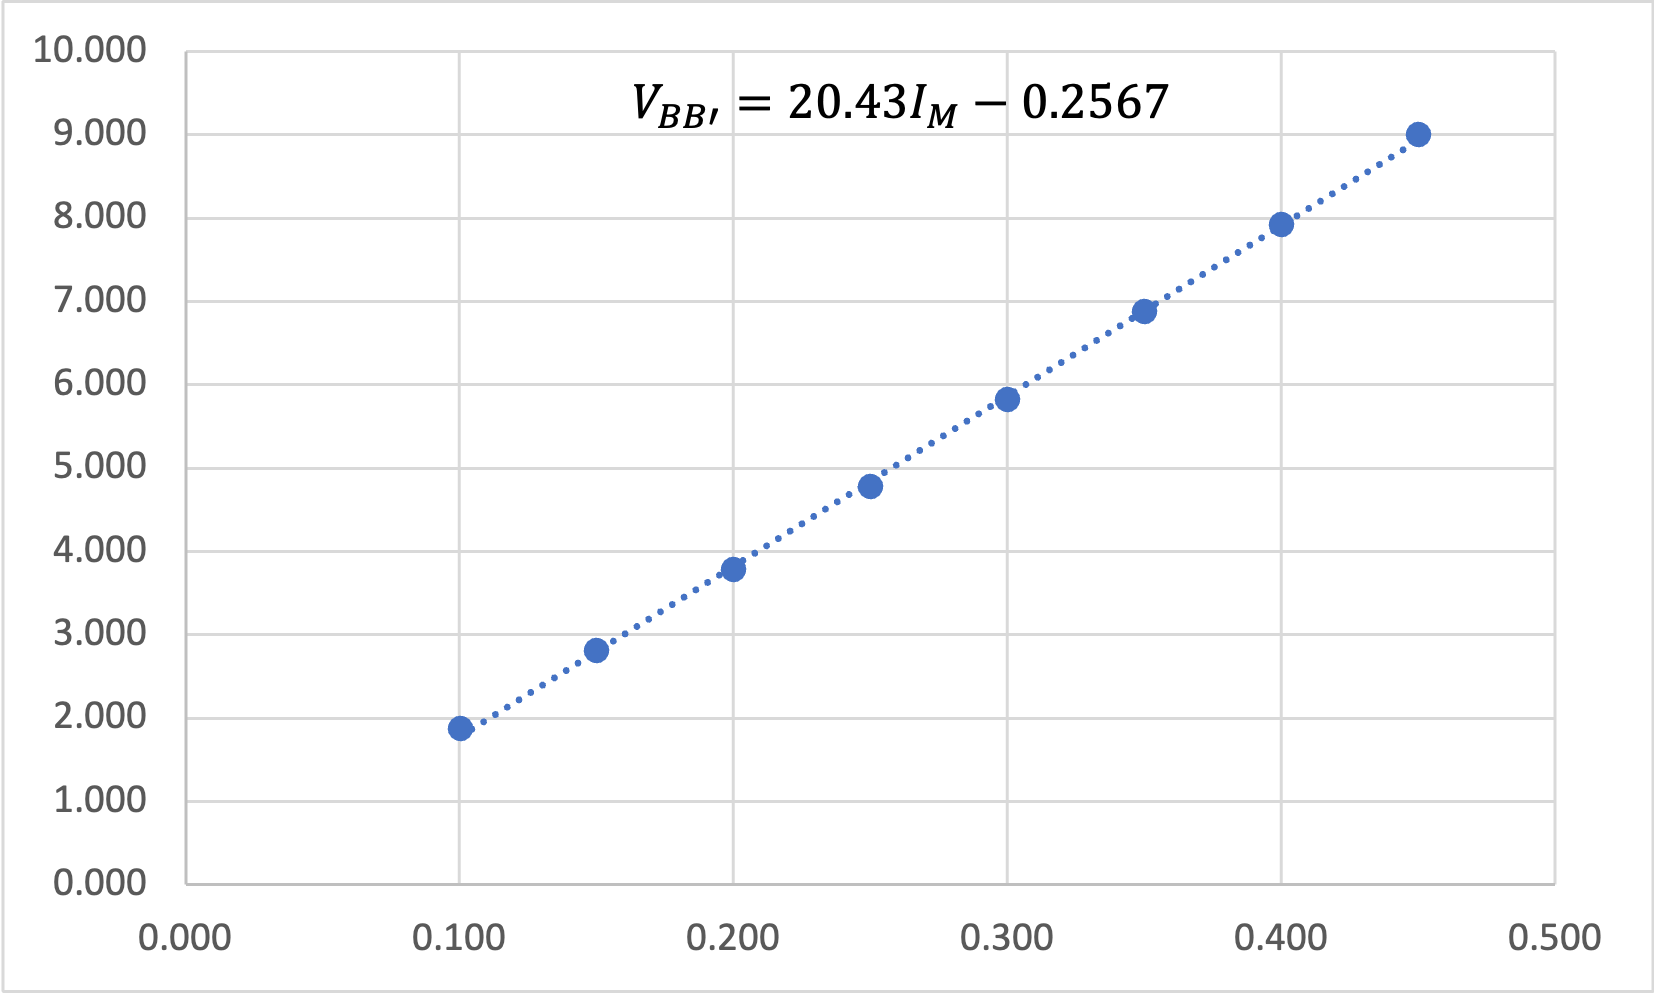
\includegraphics[scale=0.7]{p3.png}
  \caption{$V_{BB'}$与$I_M$的关系}
\end{figure}
在图3中,由
\[V_{BB'} = k_1I_S\]
\[k_1 = \frac{R_HI_M}{d}\times 0.36\mathrm{T/A}\]

得:
\[R_H = 6.306\times 10^{-3}\mathrm{m^3/C}\]

在图4中,由
\[V_{BB'} = k_2I_M\]
\[k_2 = \frac{R_HI_S}{d}\times 0.36\mathrm{T/A}\]

得:
\[R_H = 6.160\times 10^{-3}\mathrm{m^3/C}\]

由
\[\frac{V}{I_S} = \frac{L}{\sigma bd}\]

可得:
\[\sigma = 25\mathrm{S/m}\]

由图2可知,洛伦兹力$\overrightarrow{F}$方向向上,因此为n型半导体,有:
\[R_H = \frac{1}{ne}\]
\[\sigma = ne\mu\]

取$R_H$为两次测量结果的平均值$6.223\times 10^{-3}\mathrm{m^3/C}$可解得:
\[n = 1.00\times 10^{21}\mathrm{m^{-3}}\]
\[\mu = 0.154\mathrm{m^2/(Vs)}\]

对于锑化铟片,由表3数据绘制散点图:

\begin{figure}[h]
  \centering
  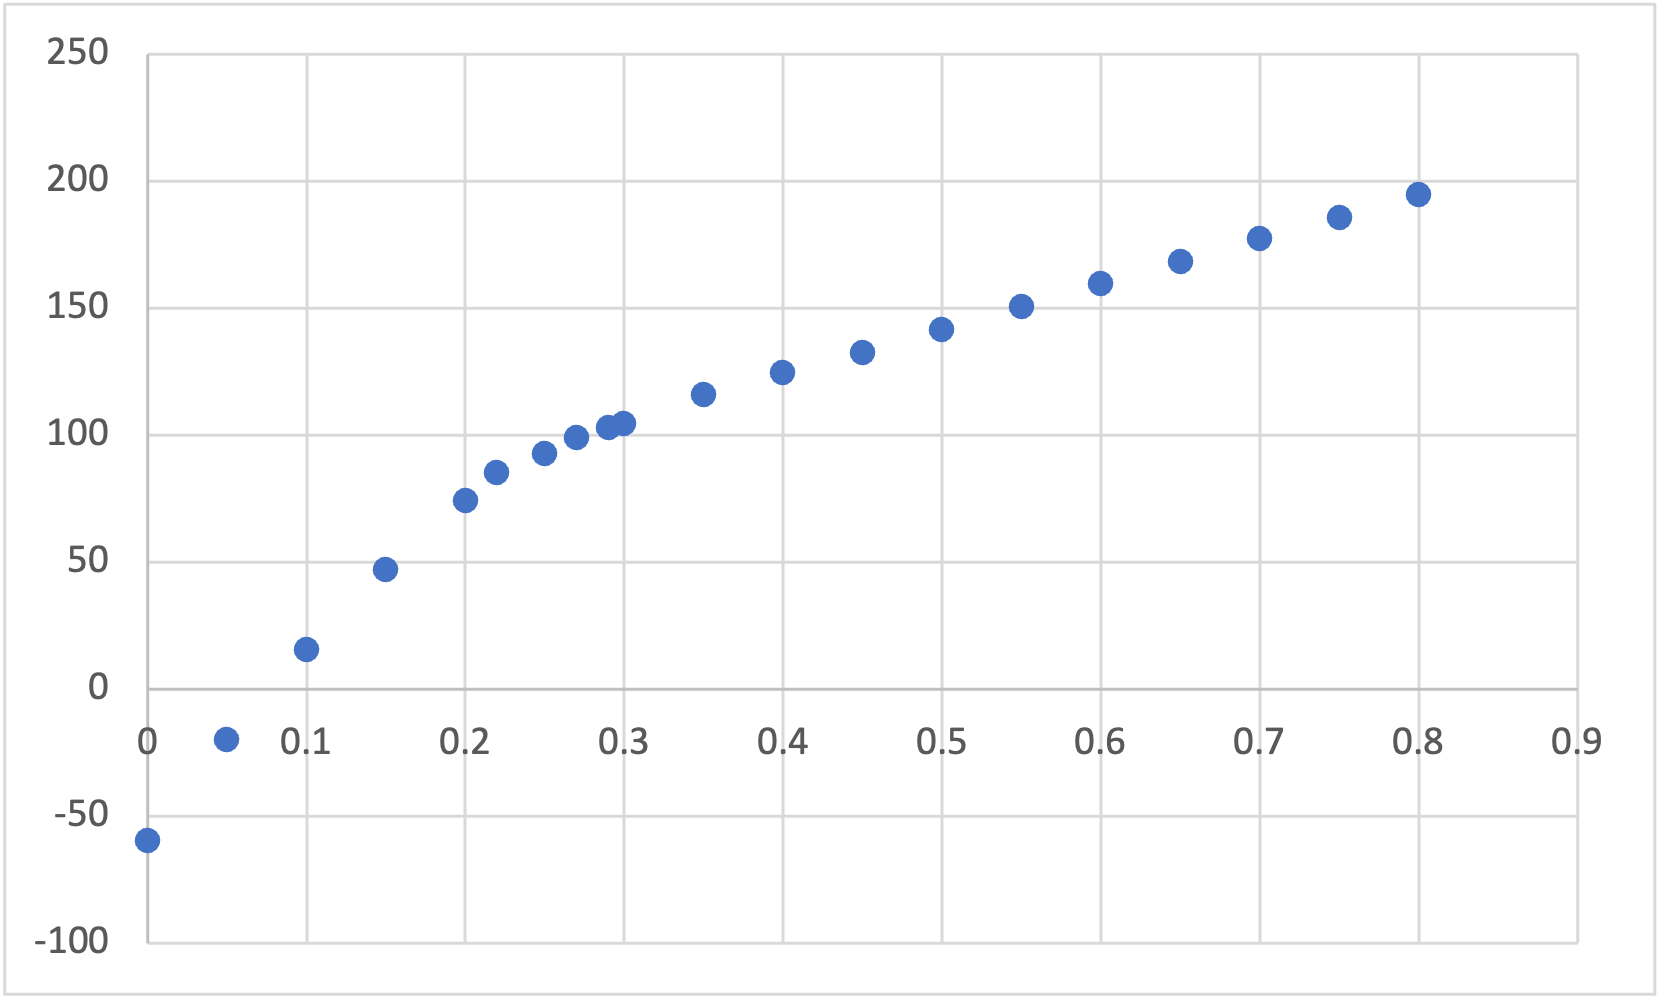
\includegraphics[scale=0.7]{p5.png}
  \caption{锑化铟片$V_H$与$I_M$关系散点图}
\end{figure}

可以发现$V_H$与$I_M$大致呈现分段的线性关系,分界点大致在$I_M=0.22\mathrm{A}$,因此分段进行线性拟合,结果如下:
\begin{figure}[h]
  \centering
  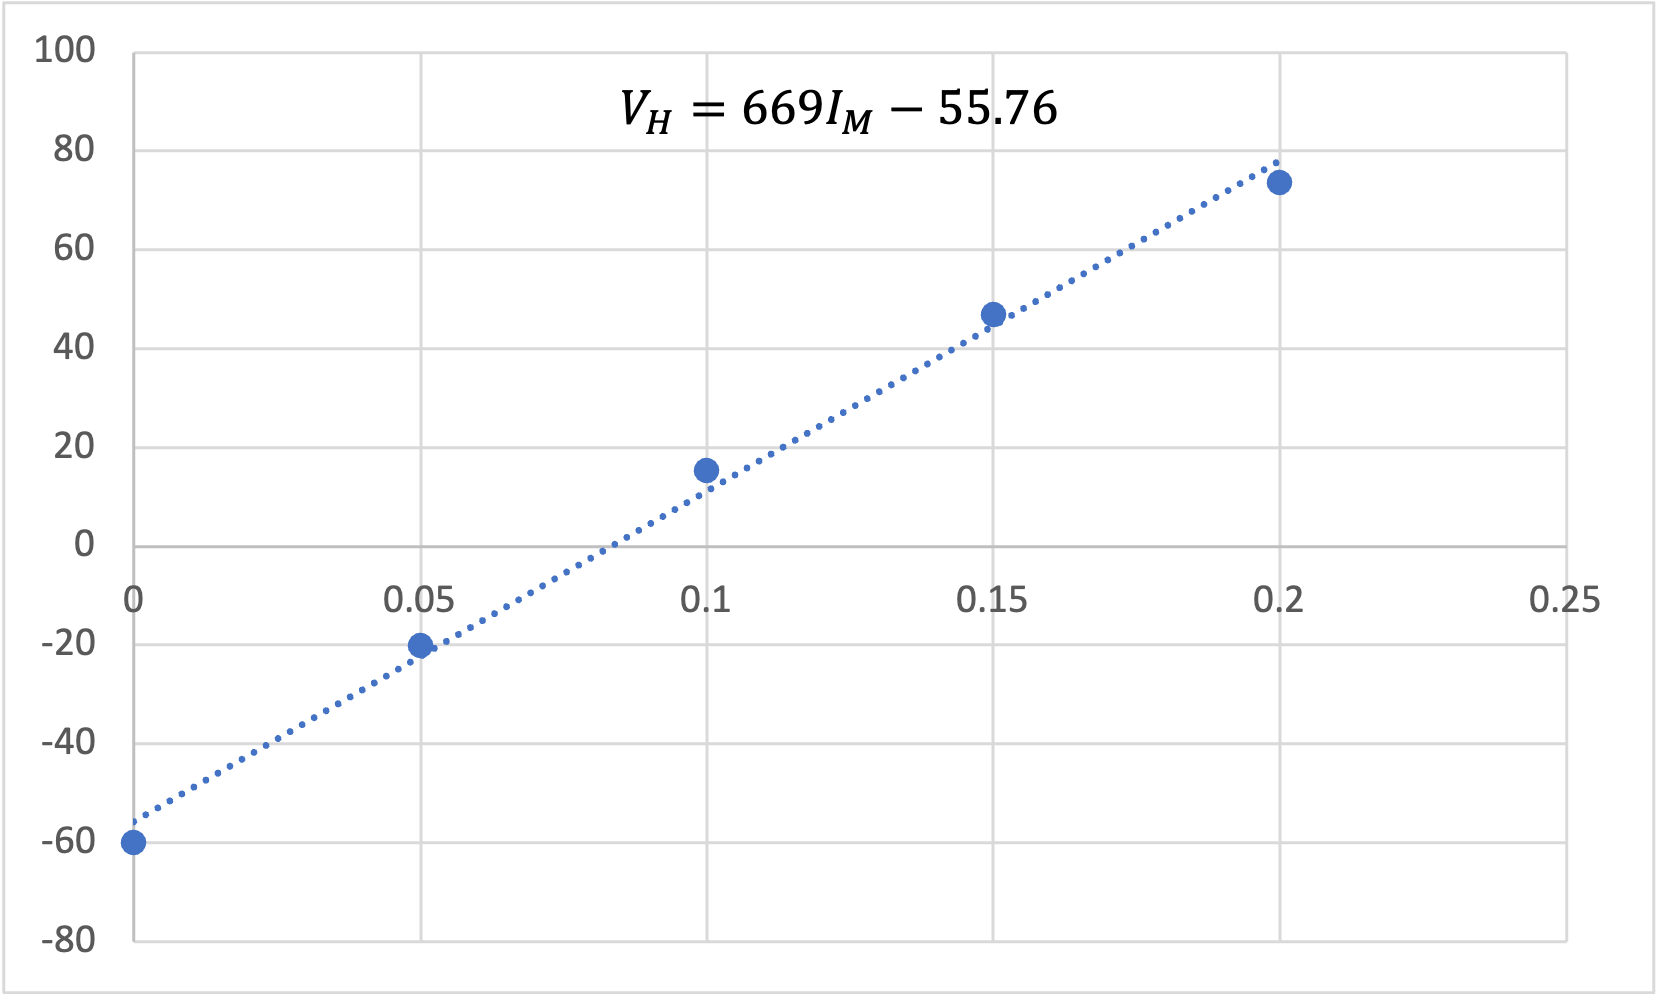
\includegraphics[scale=0.7]{p6.png}
  \caption{$I_M<0.22\mathrm{A}$}
\end{figure}

由
\[k_3 = \frac{R_{H_1}I_S}{d}\times 0.36\mathrm{T/A}\]

得:
\[R_{H_1} = 0.929\mathrm{m^3/C}\]

\begin{figure}[h]
  \centering
  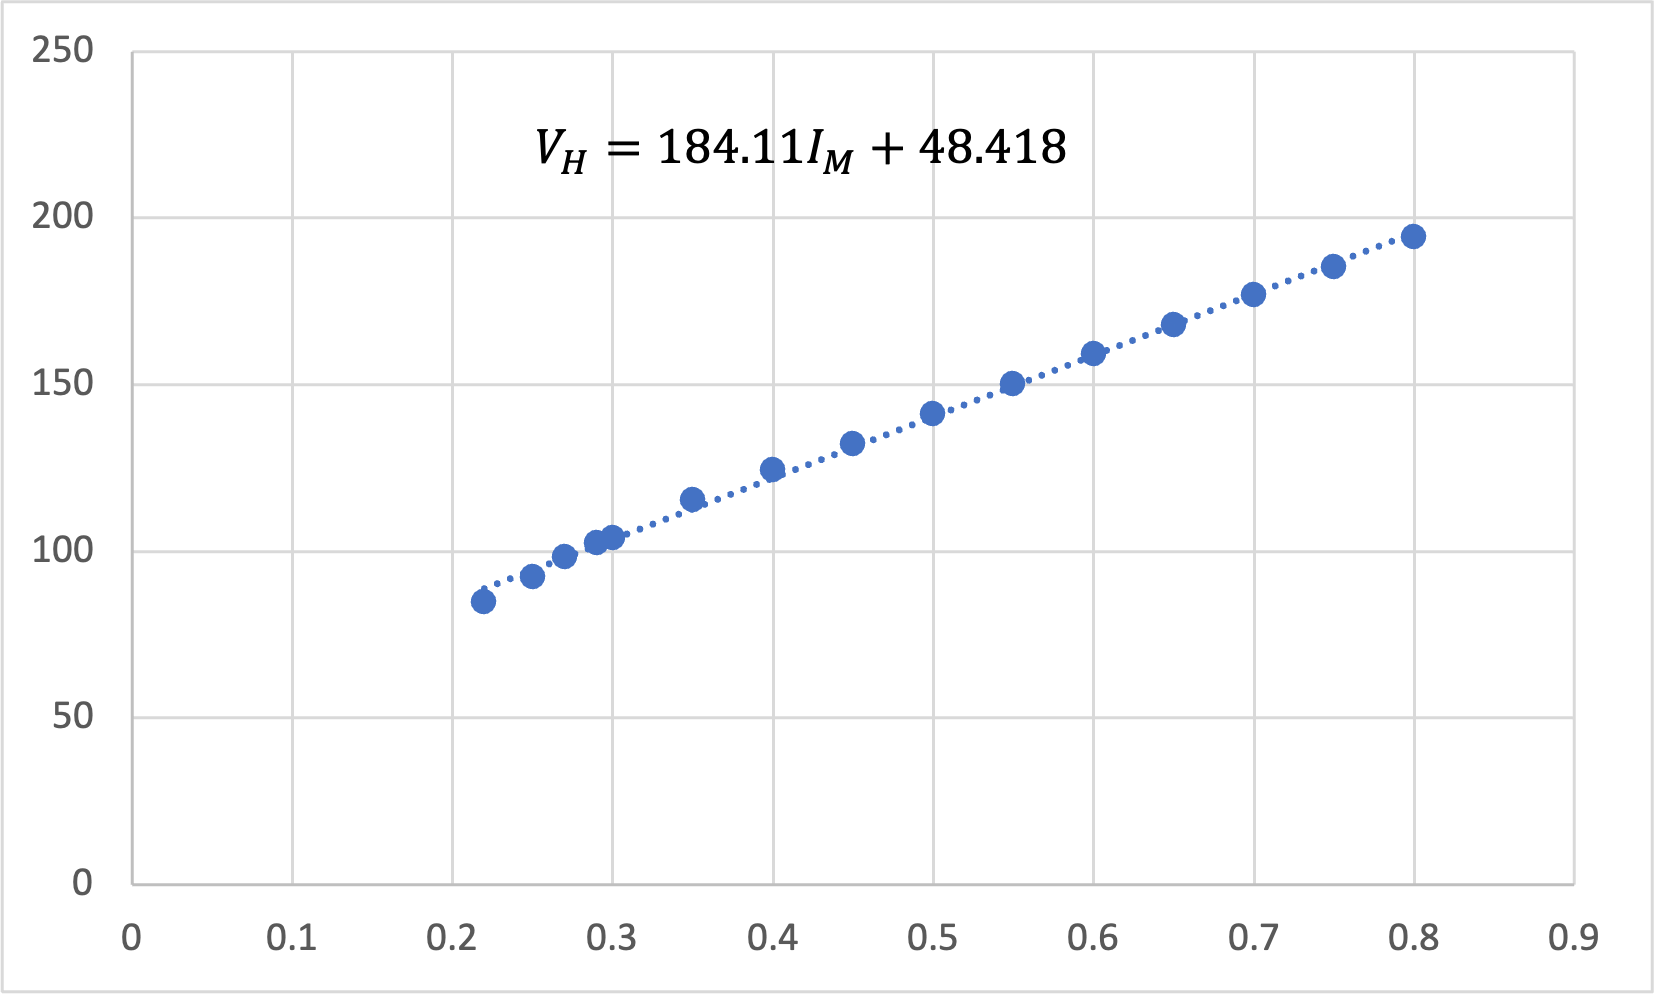
\includegraphics[scale=0.7]{p7.png}
  \caption{$I_M>0.22\mathrm{A}$}
\end{figure}

由
\[k_4 = \frac{R_{H_2}I_S}{d}\times 0.36\mathrm{T/A}\]

得:
\[R_{H_2} = 0.256\mathrm{m^3/C}\]

\subsection{误差分析}
本实验的误差主要来源于以下几点:
\begin{enumerate}
  \item 测量时仪器读数不稳定;
  \item 电极焊接不对称导致的不等位电动势;
  \item 载流子速度不一致,其横向分布也不一致,同时高速载流子温度较高,从而形成温差电动势$V_E$
\end{enumerate}

同时注意到测量锑化铟片霍尔系数时,$I_M=0$时测得电压并不为0(且绝对值并不小),推测其原因可能是上述第2点,考虑到本实验主要关心线性拟合的斜率,这对结果无显著影响(希望如此).
\bibliography{math}

\end{document}
\iffalse
\begin{figure}[h]
    \centering
    \includegraphics[scale=0.5]{name.png}
    \caption{name}
\end{figure}
\fi
